\documentclass[letterpaper, 11pt]{article}
\usepackage{amsmath}
\usepackage{mathtools}
\usepackage{amssymb}
\usepackage{float}
\usepackage{inputenc}
\usepackage[left=2cm, right=2cm, top=2cm, bottom=2cm]{geometry}
\usepackage{graphicx}
\usepackage{float}
\usepackage{caption}
\usepackage{extarrows}
\usepackage{xcolor}
\usepackage{lscape}
\usepackage{pdflscape}
\usepackage{pdfpages}
\usepackage{multicol}
\usepackage{leftindex}
\usepackage{nicefrac, xfrac}
\usepackage{algorithm2e}
\SetKwComment{Comment}{/* }{ */}
%\RestyleAlgo{ruled}
\usepackage{mathtools}
\usepackage{hyperref}
\hypersetup{
    colorlinks=false,
    }

% Listings
\usepackage{listings}
\usepackage{color}
\definecolor{mygreen}{rgb}{0,0.6,0}
\definecolor{mygray}{rgb}{0.5,0.5,0.5}
\definecolor{mymauve}{rgb}{0.58,0,0.82}

\lstset{
  backgroundcolor=\color{white},   % choose the background color; you must add \usepackage{color} or \usepackage{xcolor}; should come as last argument
  basicstyle=\small\ttfamily,        % the size of the fonts that are used for the code
  breakatwhitespace=false,         % sets if automatic breaks should only happen at whitespace
  breaklines=true,                 % sets automatic line breaking
  captionpos=t,                    % sets the caption-position to bottom
  commentstyle=\color{mygreen},    % comment style
  deletekeywords={...},            % if you want to delete keywords from the given language
  escapeinside={\%*}{*)},          % if you want to add LaTeX within your code
  extendedchars=true,              % lets you use non-ASCII characters; for 8-bits encodings only, does not work with UTF-8
  firstnumber=1,                % start line enumeration with line 1000
  frame=false,	                   % adds a frame around the code
  keepspaces=true,                 % keeps spaces in text, useful for keeping indentation of code (possibly needs columns=flexible)
  keywordstyle=\color{blue},       % keyword style
  language=Python,                 % the language of the code
  morekeywords={*,...},            % if you want to add more keywords to the set
  numbers=none,                    % where to put the line-numbers; possible values are (none, left, right)
  numbersep=5pt,                   % how far the line-numbers are from the code
  numberstyle=\tiny\color{mygray}, % the style that is used for the line-numbers
  rulecolor=\color{black},         % if not set, the frame-color may be changed on line-breaks within not-black text (e.g. comments (green here))
  showspaces=false,                % show spaces everywhere adding particular underscores; it overrides 'showstringspaces'
  showstringspaces=false,          % underline spaces within strings only
  showtabs=false,                  % show tabs within strings adding particular underscores
  stepnumber=5,                    % the step between two line-numbers. If it's 1, each line will be numbered
  stringstyle=\color{mymauve},     % string literal style
  tabsize=4,	                   % sets default tabsize to 2 spaces
  title=\lstname                   % show the filename of files included with \lstinputlisting; also try caption instead of title
}


% NewCommands
\newcommand{\peq}{ \mathrel{+}= }
\newcommand{\muleq}{ \mathrel{*}= }
\newcommand{\sign}{ \text{sign}}
\newcommand{\bm}[1]{\begin{bmatrix} #1 \end{bmatrix}}
\newcommand{\mat}[1]{\begin{matrix} #1 \end{matrix}}
\newcommand{\lx}[2]{\leftindex #1 {#2}}
\newcommand{\norm}[1]{\left\lvert #1 \right\rvert}
\newcommand{\itbf}[1]{\textit{\textbf{#1}}}
\newcommand{\mdet}[1]{\norm{\begin{matrix} #1 \end{matrix}}}
\newcommand{\pbox}[1]{\fbox{\begin{minipage}{\textwidth} #1 \end{minipage}}}
\newcommand{\lstln}[1]{\lstinline|#1|}
\newcommand{\lr}[1]{\left( #1 \right)}
\newcommand{\lrb}[1]{\left[ #1 \right]}
\newcommand{\lrf}[1]{\left\{ #1 \right\}}
\newcommand{\adj}{\text{adj}}


\title{Modelling SCR system dynamics}
\author{Sesha Charla}
\date{\today}


\begin{document}
\maketitle
\tableofcontents
\newpage
%===============================================================================
\section{Introduction}

Diesel engine after-treatment systems are engineered to diminish the emission of
harmful gases such as $NO_x$ and $CO$ from exhaust gases. The SCR-ASC system
chemically converts $NO_x$ into $N_2$ and $H_2O$, utilizing ammonia as a reducing agent
in the presence of a catalyst. This catalytic conversion process is regulated to
decrease the levels of ammonia in the exhaust, known as Ammonia Slip, through
two methods. The first is feedback control, which adjusts the urea injection
rate based on the exhaust $NO_x$ concentrations. The second method involves an
additional catalytic reaction, the ASC (Ammonia Slip Catalysis), which is
designed to oxidize any excess ammonia at the end of the SCR bed.
Figure~\ref{fig:exhaust_scheme} shows a schematic of the SCR system. The
catalyst aging is a critical issue in the SCR-ASC system, as it can lead to
reduction in the efficacy of conversion and increased ammonia slip. A
fault detection system that can detect the aging of the catalyst would provide
better control over the maintenance of the system and improve the overall
reduction in emissions.

\begin{figure}[ht]
    \centering
    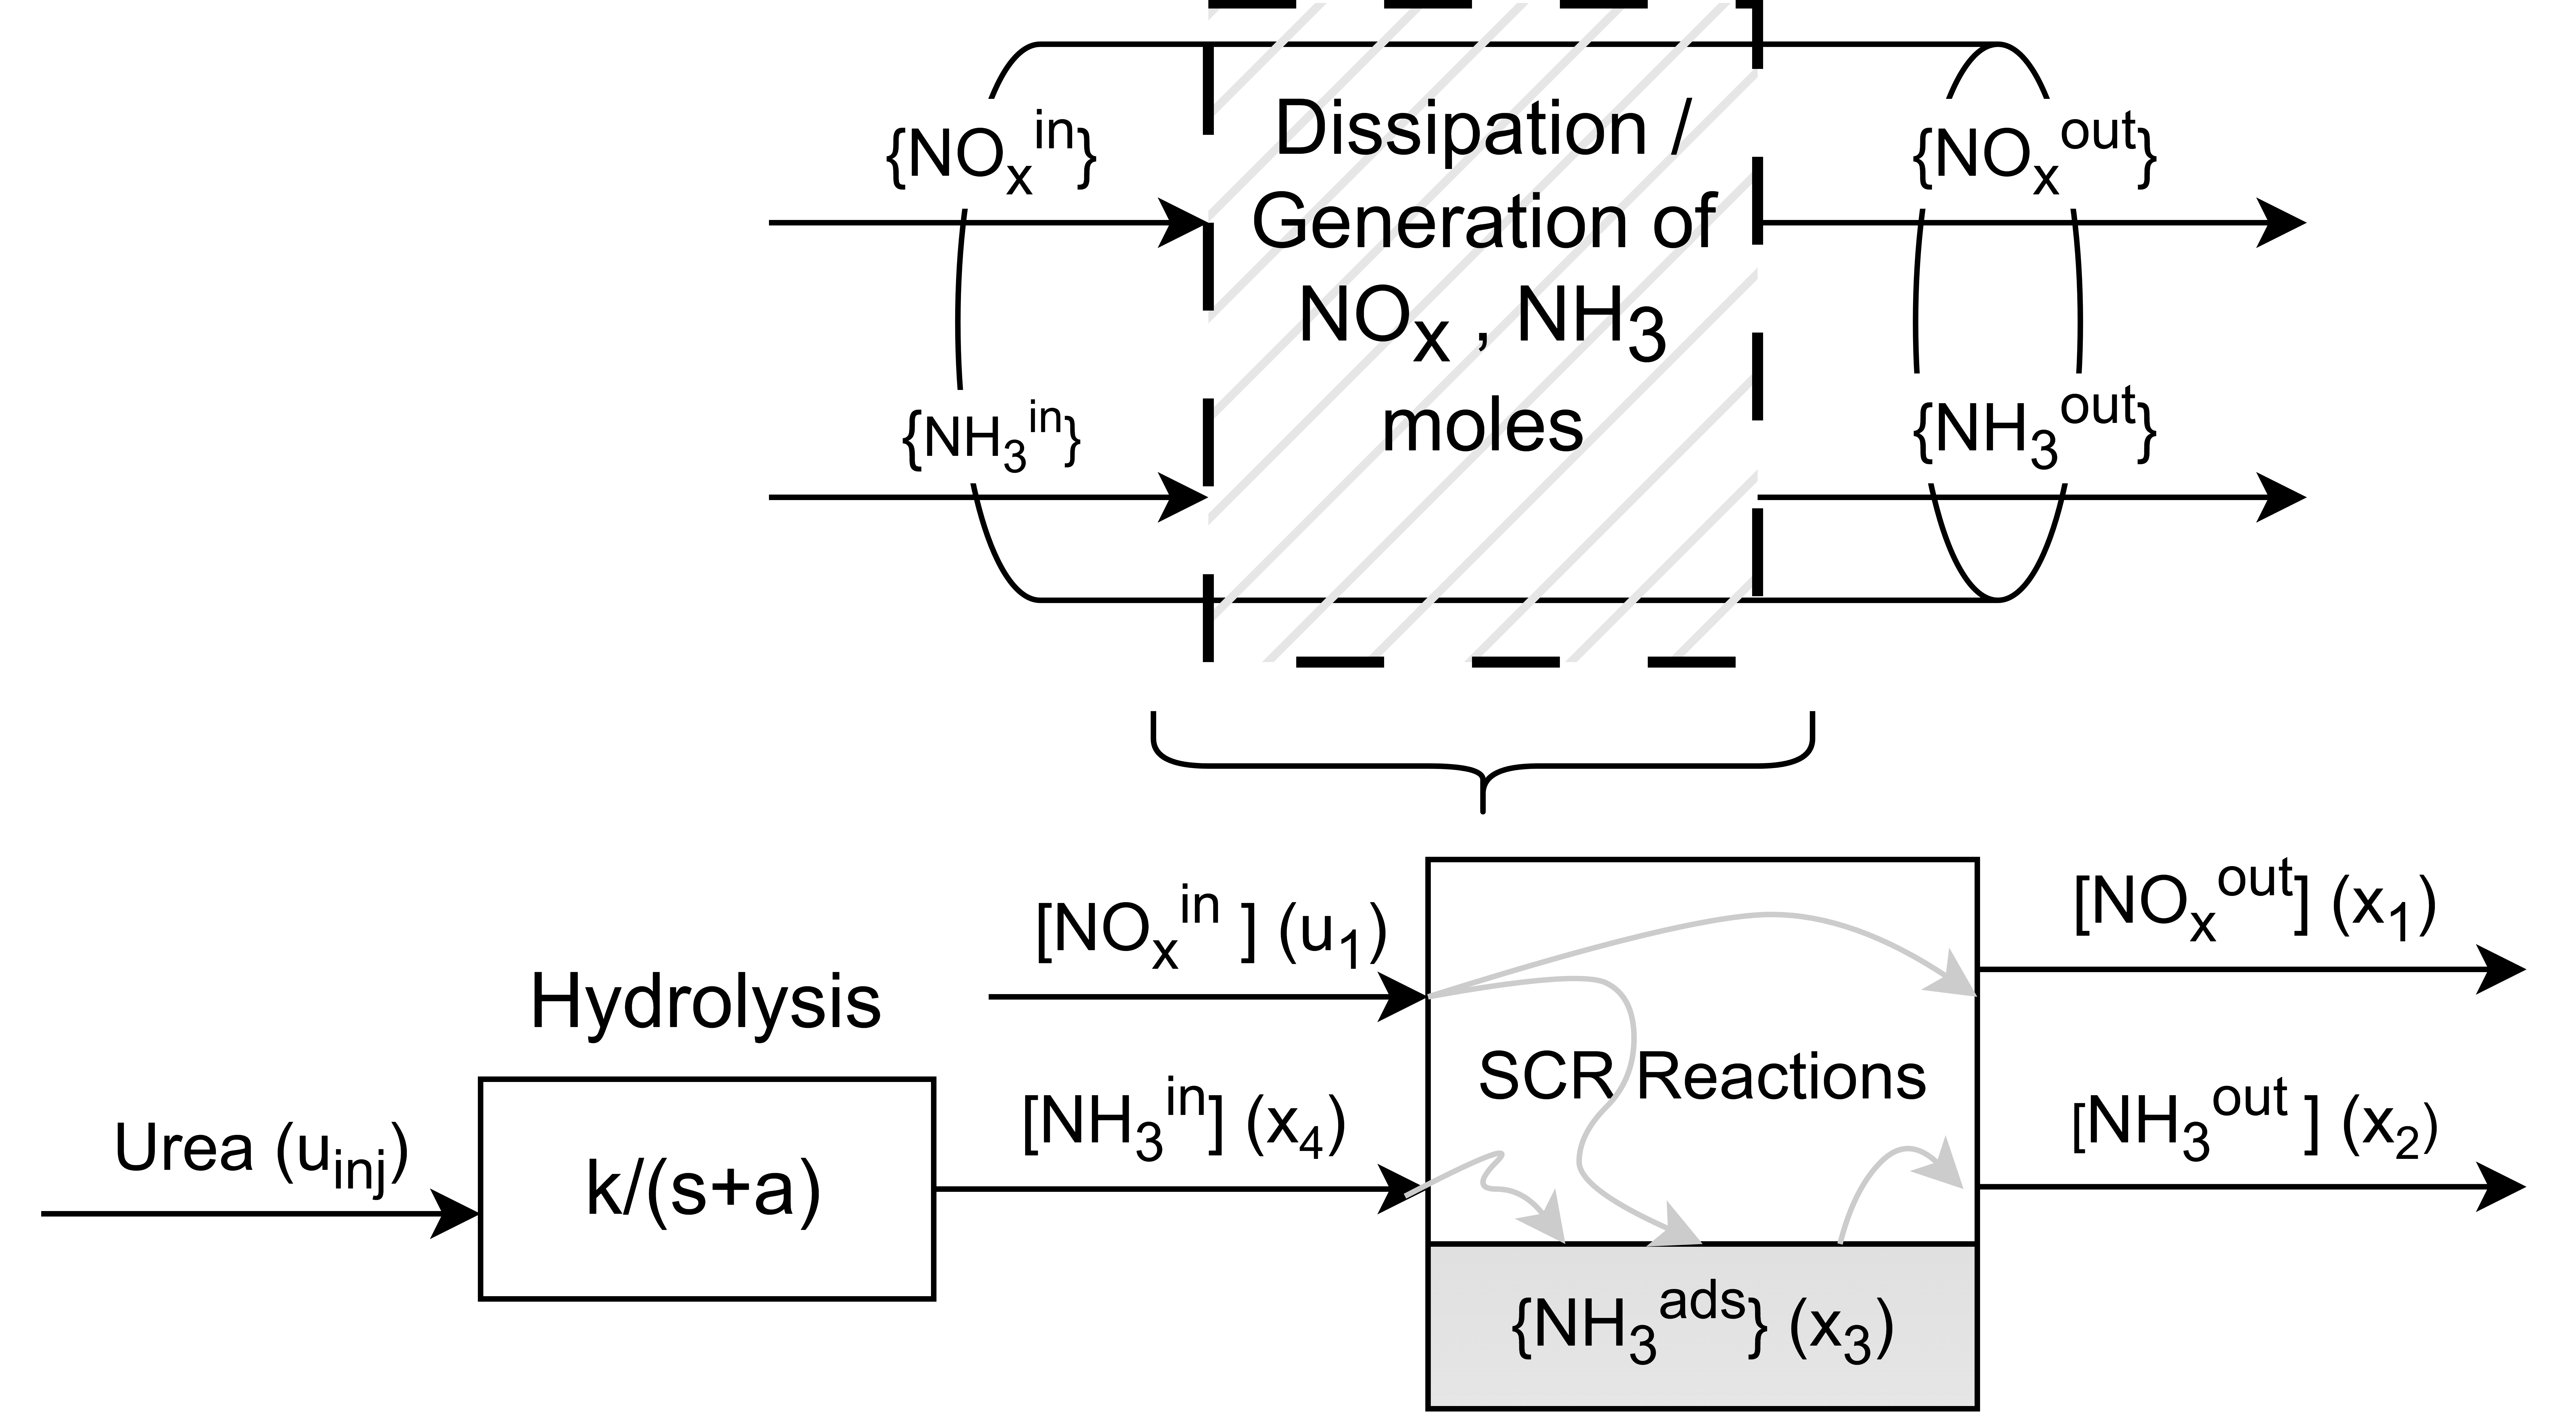
\includegraphics[width=0.45\textwidth]{./figs/scr_sys/SCR_sys.png}
    \caption{Schematic of the SCR system}
    \label{fig:exhaust_scheme}
\end{figure}


Thus, modern diesel after-treatment systems, particularly those that integrate Selective Catalytic Reduction (SCR) with
Ammonia Slip Catalyst (ASC), necessitate advanced on-board diagnostics (OBD) tools for accurate assessment of SCR
degradation levels. However, the effectiveness of traditional OBD approaches for this purpose has been impeded by the
absence of model validation with real-world catalyst degradation data and the limitations imposed by existing commercial
$NO_x$ sensors' cross-sensitivity to ammonia.

Numerous studies have been conducted on modeling the SCR-ASC systems and their control (\cite{yuan2015diesel}). A
prevalent modeling approach is to approximate the PDE model from the plug flow reactor assumption into a set of ODEs
using the idealization of the plug-flow reactor into a sequence of CSTRs (\cite{hsieh2011development}, and
\cite{nova2014urea}). This discretization requires at least 2 CSTRs to capture the system dynamics and causality,
thereby increasing the model order. Moreover, the reactions considered are generally confined to selected SCR and ASC
reactions. The single CSTR approach was first justified in \cite{devarakonda2008adequacy} and a nonlinear model was
developed using these assumptions, which was then linearized for feedback control design (\cite{devarakonda2009model}).
With this model, observers were designed to estimate the states corresponding to the catalyst's storage
(\cite{ma2017observer}, \cite{jain2020term}). A method for detecting the catalyst's aging by observing the change in the
maximum storage capacity of the catalyst, modeled as an exponential function of temperature, was also proposed in
\cite{ma2017observer}. A common theme in these studies is the resulting non-convex, nonlinear parameter estimation
problem. Moreover, these studies assume the availability of all the gaseous states at the tail-pipe to eliminate the
effects of cross-sensitivity of the $NO_x$ sensors, which is not always the case in real-world applications. One other
fundamental issue with a single cell CSTR assumption is that it results in the causality reversal at the reaction rates
as CSTR inherently assumes that the output concentrations are the same as CSTR's accumulator concentrations.


The existing models for control and estimation of diesel-engine SCR-ASC dynamics spur the need for a "low-order",
"high-fidelity" model capable of diagnostics.

One of the fundamental assumptions in the diesel engine SCR-ASC modelling, CSTR, reverts the causality in the reaction
rate constants, when the model order is reduced by considering a single cell. The present work circumvents the problem
by discarding the CSTR assumption and modelling the time evolution of the sensor signals when a "plug" or "parcel" of
the exhaust gasses flows through the chamber.

Such a time evolution introduces constraints on the model due to sampling limitations. To capture the transient
dynamics, the sampling time should be significantly smaller than the "residence time" of the reactants inside the
SCR-ASC chamber. If that is not the case as is the situation with the present available test and truck data, time integrated states assuming zero-order holds during the transients need to be introduced into the model and the input-output model can be derived from the resulting state-space model.

The modelling approach involves following the evolution of the measurement signals at the input and the output of the
system. As the plug of fluid flows through the chamber, these measurements can be correlated based on the conservation
of moles within the fluid plug.

%===============================================================================
% \newpage
% \section{SCR Reaction Kinetics}

\subsection{SCR Reactions}
Eley Rideal reaction mechanism \cite{hsieh2011development}
\cite{yuan2015diesel}, \cite{nova2014urea} is considered for the interpreting
the SCR reactions. The mechanism involves the following reactions:

\begin{align*}
    NH_2 - CO - NH_2 (liquid) &\longrightarrow NH_2 - CO - NH_2^* + x H_2 O
                & &[\text{AdBlue evaporation}] \\
    NH_2 - CO - NH_2^*  &\longrightarrow  HNCO + NH_3
                & &[\text{Urea decomposition}] \\
    HNCO + H_2O &\longrightarrow NH_3 + CO_2
                & &[\text{Isocynic acid hydrolysis}] \\
    %===
    NH_3 + \theta_{free} &\longleftrightarrow NH_3(ads)
                         & &[\text{Ammonia Adsorption/Desorption}]\\
    %===
    4 NH_3 (ads) + 4 NO + O_2 &\longrightarrow 4 N_2 + 6 H_2O
                              & &[\text{Standard SCR reaction}]\\
    %===
    2 NH_3 (ads) +  NO + N O_2 &\longrightarrow 2 N_2 + 3 H_2O
                              & &[\text{Fast SCR reaction}]\\
    %===
    4 NH_3 (ads) + 3N O_2 &\longrightarrow 3.5 N_2 + 6 H_2O
                              & &[\text{Slow SCR reaction}]\\
    %===
    4 NH_3 + 3 O_2 &\longrightarrow 2 N_2 + 6 H_2O
                         & &[\text{AMOX with/without ASC}]\\
    4 NH_3 + 5 O_2 &\longrightarrow 4 NO + 6 H_2 O
                         & &[\text{AMOX with/without ASC}]\\
    2 NH_3 + 2 O_2 &\longrightarrow N_2O + 3 H_2O
                         & &[\text{AMOX with/without ASC}]\\
    %==
    2 NO + O_2 &\longrightarrow 2 NO_2
                        & &[\text{NO oxidation}]
\end{align*}


The PDE model for SCR reaction kinematics \cite{nova2014urea} is reduced to ODE model \cite{devarakonda2008adequacy} using by assuming "continuous stirred tank reactor (CSTR)" model (Control volume approach).

Further, in order to keep the model order reasonably low only the following
three reactions are considered:
\begin{enumerate}
    \item Standard SCR reaction:
    \begin{align}
        4 NH_3 (ads) + 4 NO + O_2 &\longrightarrow 4 N_2 + 6 H_2O \label{eqn::std_scr}
    \end{align}
    \item Ammonia Oxidation:
    \begin{align}
        4 NH_3 + 3 O_2 &\longrightarrow 2 N_2 + 6 H_2O \label{eqn::amox}
    \end{align}
    \item Ammonia Adsorption/Desorption:
        \begin{align}
            NH_3 + \theta_{free} &\longleftrightarrow NH_3(ads)
            \label{eqn::ads}
        \end{align}
\end{enumerate}

\subsection{General reaction kinetics}
For a stoichiometric reaction of the following form:
\begin{align*}
    a A + b B \longrightarrow c C + d D
\end{align*}
We have the reaction rate \cite{chem_kine}:
\begin{align}
    r &= -\frac{1}{a} \frac{d [A]}{dt}
       = -\frac{1}{b} \frac{d [B]}{dt}
       = \frac{1}{c}  \frac{d [C]}{dt}
       = \frac{1}{d}  \frac{d [D]}{dt}
       \label{eqn::react_rate}\\
    r &= k [A]^m [B]^n
        \label{eqn::rate}
\end{align}
Where,
\begin{align*}
    [\bullet] &- \text{Concentration of the reactant } \bullet\\
    k &- \text{Rate constant}\\
    m, n &- \text{Constant exponents, ($m+n$) is the order of reaction}\\
\end{align*}
In the subsequent derivations, the exponents in the rate equations are limited
to either zero or 1 $m, n \in \{0, 1\}$ (This is consistent with the assumption
that reaction rates are proportional to gas-phase concentrations from \cite{devarakonda2009model}).

The rate constant can be determined using \itbf{Arrhenius equation}:
\begin{align}
    k &= A e^{E_a/RT}
    \label{eqn::arrh}
\end{align}
\begin{align*}
    \text{Where,} \quad &\\
    A &- \text{Pre-exponential factor}\\
    E_a &- \text{Activation energy}\\
    T &- \text{Temperature}\\
    R &- \text{Universal gas constant}
\end{align*}
\subsubsection{Effects of temperature change on rate constant}
We have the Arrhenius equation:
\begin{align}
    k &= A e^{-E_a/RT}
\end{align}
\begin{align*}
    \implies \delta k &= \delta T A \lr{\frac{E_a}{RT^2}} e^{-E_a/RT} = \delta T k \lr{\frac{E_a}{RT^2}}
\end{align*}
In general, $E_a$ is several orders of magnitude greater than the other
parameters. Thus, small change in temperature gets amplified as the change in
the rate-constant.

Also, we have the first-order tayler approximation for the rate-constant
variation with temperature:
\begin{align*}
    k(T_0 + \delta T) &\approx \bar k(T_0) + \frac{E_a}{RT_0^2} \bar k(T_0) \delta T
\end{align*}
\begin{align}
    k(\delta T) &\approx \bar k + p \bar k \delta T
\end{align}
Where,
\begin{align*}
    p &= \frac{E_a}{RT_0^2}
\end{align*}
This form would be more amenable to parameter estimation despite introducing
approximation errors.



%===============================================================================
\subsection{Eley-Rideal Mechanism}
In this mechanism, proposed in 1938 by D. D. Eley and E. K. Rideal, only one of
the molecules adsorbs and the other one reacts with it directly from the gas
phase, without adsorbing ("non-thermal surface reaction") \cite{eley_rideal}.

\itbf{Note:} The concentration $(\lrb{\bullet})$ can mean either surface
concentration or volumetric concentration based on the context. The
rate-constants take care of the necessary unit conversions.

\begin{align*}
    A^{g} + \Theta_{free} &\rightleftharpoons A^{ads}  \qquad (k_1, k_{-1})\\
    A^{ads} + B^{g} &\longrightarrow Products \qquad (k)
\end{align*}

We have the rate of the second reaction:
\begin{align*}
    r &= k \con{A^{ads}} \con{B}
\end{align*}
Thus,
\begin{align*}
    \frac{d \con{A^{ads}}}{dt} &= k_1 [A] \con{\Theta - \mol{A^{ads}}} - k_{-1} \con{A^{ads}} - k \con{A^{ads}} \lrb{B}
\end{align*}

\itbf{Note:} If the volume of the reaction chamber is constant. The
concentration $\con{.}$ can be replaced with the number of moles $\mol{.}$ without changing the structure of the equations. Only the values of the rate
constants change accommodating the change in units and the volume/area when required.

Thus,
\begin{align}
    \frac{d \mol{A^{ads}}}{dt} &= k_1 [A] \lr{\Theta - \mol{A^{ads}}}
                                - k_{-1} \mol{A^{ads}}
                                - k \mol{A^{ads}} \con{B}
    \label{eqn::eley_rideal}
\end{align}

Where,
\begin{align*}
    \Theta &- \text{Molar storage capacity of the catalyst:}\\
           &\qquad \text{The total number of moles that can be adsorbed on to the surface}\\
    \lrb{\bullet} &= \text{Concentration of $\bullet$}\\
    \lrf{\bullet} &= \text{Number of moles of $\bullet$}
\end{align*}

%

\subsection{Reaction Rates}
\itbf{Assumptions:}
\begin{enumerate}
\item The reaction rates are only functions of gas-phase concentrations of $NO$,
$NH_3$, the adsorbed Ammonia and the available adsorption sites $\lr(\Theta)$.

\item The concentration rates are converted into molar-rate so that the
mass balance in control volume approach (CSTR) can be performed.

\item A lower order Tayler approximation is assumed to model the temperature
effects in rate constant.

\item As the volume of the reaction chamber is constant. The concentration
    $\lrb{.}$ is replaced with the number of moles $\lrf{.}$ without changing
        the structure of the equations for convenience. Only the values of the
        rate constants change accommodating the change in units and the
        volume/area when required.
\end{enumerate}

\begin{enumerate}
\item Standard SCR Reaction (\ref{eqn::std_scr}):
$ NH_3 ^{(ads)} +  NO + (1/4) O_2 \longrightarrow  N_2 + (3/2) H_2O$
\begin{align}
    r_1 &= k_1 [NO_x^{in}] \mol{NH_3^{ads}}\\
    k_1 &= A_1 e^{\frac{-E_1}{RT}} \approx \bar k_1 + p_1 \bar k_1 \delta T \qquad \lrb{p_1 = \frac{E_1}{R T_0^2}}
\end{align}

\item Ammonia Oxidation (\ref{eqn::amox}):
    $ NH_3 + (3/4) O_2 \longrightarrow (1/2) N_2 + (3/2) H_2O$
\begin{align}
    r_2 &= k_2 \mol{NH_3^{in}}\\
    k_2 &= A_2 e^{\frac{-E_2}{RT}} \approx \bar k_2 + p_2 \bar k_2 \delta T \qquad \lrb{p_2 = \frac{E_2}{R T_0^2}}
\end{align}

\item Ammonia Adsorption/Desorption (\ref{eqn::ads}):
$NH_3 + \theta_{free} \rightleftharpoons  NH_3^{(ads)}$
\begin{enumerate}
\item Forward:
\begin{align}
    r_{3F} &= k_{3F} \con{NH_3^{in}} \lr{\Theta - \mol{NH_3^{ads}}}\\
    k_{3F} &= A_{3F} e^{\frac{-E_{3F}}{RT}} \approx \bar k_{3F} + p_{3F} \bar k_{3F} \delta T \qquad \lrb{p_{3F} = \frac{E_{3F}}{R T_0^2}}
\end{align}

\item Reverse:
\begin{align}
    r_{3R} &= k_{3R} \mol{NH_3^{ads}}\\
    k_{3R} &= A_{3R} e^{\frac{-E_{3R}}{RT}} \approx \bar k_{3R} + p_{3R} \bar k_{3R} \delta T \qquad \lrb{p_{3R} = \frac{E_{3R}}{R T_0^2}}
\end{align}
\end{enumerate}
\end{enumerate}

Where,
\begin{align*}
    \Theta &- \text{Ammonia storage capacity} (moles)\\
    E_i &- \text{Activation Energy of $i^{th}$ reaction}\\
    A_i &- \text{Pre-exponential factor}\\
    R &- \text{Universal gas constant}\\
    T &- \text{Temperature}\\
\end{align*}


% %===============================================================================
% \newpage
% \input{secs/3_urea_dosing.tex}
% %===============================================================================
% \newpage
% \input{secs/4_3state_model.tex}
% %===============================================================================
% \newpage
% \input{secs/5_adsorption_model.tex}
% %===============================================================================
% \newpage
% \input{secs/6_control_form.tex}
% % ==============================================================================
% \newpage
% \input{secs/7_cross_sensitivity_est.tex}
% %===============================================================================
% \newpage
% \input{secs/8_linear_model_identification.tex}
% % ==============================================================================
% \newpage
% \input{secs/9_DynamicModelDevelopment.tex}
% \newpage
% \section{Appencix}
% \input{secs/apx-1_4state_model.tex}
% \input{secs/apx-2_kaushal_model.tex}
\newpage
\nocite{}
\bibliographystyle{unsrt}
\bibliography{refs}

\end{document}
